\documentclass[a4paper,11pt]{book}
%\documentclass[a4paper,twoside,11pt,titlepage]{book}
\usepackage{listings}
\usepackage[utf8]{inputenc}
\usepackage[spanish]{babel}

% \usepackage[style=list, number=none]{glossary} %
%\usepackage{titlesec}
%\usepackage{pailatino}

\decimalpoint
\usepackage{dcolumn}
\newcolumntype{.}{D{.}{\esperiod}{-1}}
\makeatletter
\addto\shorthandsspanish{\let\esperiod\es@period@code}
\makeatother


%\usepackage[chapter]{algorithm}
\RequirePackage{verbatim}
%\RequirePackage[Glenn]{fncychap}
\usepackage{fancyhdr}
\usepackage{graphicx}
\usepackage{afterpage}

\usepackage{longtable}

\usepackage[pdfborder={000}]{hyperref} %referencia

% ********************************************************************
% Re-usable information
% ********************************************************************
\newcommand{\myTitle}{Título del proyecto\xspace}
\newcommand{\myDegree}{Grado en Ingeniería Informática\xspace}
\newcommand{\myName}{Nombre Apllido1 Apellido2 (alumno)\xspace}
\newcommand{\myProf}{Nombre Apllido1 Apellido2 (tutor1)\xspace}
\newcommand{\myOtherProf}{Nombre Apllido1 Apellido2 (tutor2)\xspace}
%\newcommand{\mySupervisor}{Put name here\xspace}
\newcommand{\myFaculty}{Escuela Técnica Superior de Ingenierías Informática y de
Telecomunicación\xspace}
\newcommand{\myFacultyShort}{E.T.S. de Ingenierías Informática y de
Telecomunicación\xspace}
\newcommand{\myDepartment}{Departamento de ...\xspace}
\newcommand{\myUni}{\protect{Universidad de Granada}\xspace}
\newcommand{\myLocation}{Granada\xspace}
\newcommand{\myTime}{\today\xspace}
\newcommand{\myVersion}{Version 0.1\xspace}


\hypersetup{
pdfauthor = {\myName (email (en) ugr (punto) es)},
pdftitle = {\myTitle},
pdfsubject = {},
pdfkeywords = {palabra_clave1, palabra_clave2, palabra_clave3, ...},
pdfcreator = {LaTeX con el paquete ....},
pdfproducer = {pdflatex}
}

%\hyphenation{}


%\usepackage{doxygen/doxygen}
%\usepackage{pdfpages}
\usepackage{url}
\usepackage{colortbl,longtable}
\usepackage[stable]{footmisc}
%\usepackage{index}

%\makeindex
%\usepackage[style=long, cols=2,border=plain,toc=true,number=none]{glossary}
% \makeglossary

% Definición de comandos que me son tiles:
%\renewcommand{\indexname}{Índice alfabético}
%\renewcommand{\glossaryname}{Glosario}

\pagestyle{fancy}
\fancyhf{}
\fancyhead[LO]{\leftmark}
\fancyhead[RE]{\rightmark}
\fancyhead[RO,LE]{\textbf{\thepage}}
\renewcommand{\chaptermark}[1]{\markboth{\textbf{#1}}{}}
\renewcommand{\sectionmark}[1]{\markright{\textbf{\thesection. #1}}}

\setlength{\headheight}{1.5\headheight}

\newcommand{\HRule}{\rule{\linewidth}{0.5mm}}
%Definimos los tipos teorema, ejemplo y definición podremos usar estos tipos
%simplemente poniendo \begin{teorema} \end{teorema} ...
\newtheorem{teorema}{Teorema}[chapter]
\newtheorem{ejemplo}{Ejemplo}[chapter]
\newtheorem{definicion}{Definición}[chapter]

\definecolor{gray97}{gray}{.97}
\definecolor{gray75}{gray}{.75}
\definecolor{gray45}{gray}{.45}
\definecolor{gray30}{gray}{.94}

\lstset{ frame=Ltb,
     framerule=0.5pt,
     aboveskip=0.5cm,
     framextopmargin=3pt,
     framexbottommargin=3pt,
     framexleftmargin=0.1cm,
     framesep=0pt,
     rulesep=.4pt,
     backgroundcolor=\color{gray97},
     rulesepcolor=\color{black},
     %
     stringstyle=\ttfamily,
     showstringspaces = false,
     basicstyle=\scriptsize\ttfamily,
     commentstyle=\color{gray45},
     keywordstyle=\bfseries,
     %
     numbers=left,
     numbersep=6pt,
     numberstyle=\tiny,
     numberfirstline = false,
     breaklines=true,
   }
 
% minimizar fragmentado de listados
\lstnewenvironment{listing}[1][]
   {\lstset{#1}\pagebreak[0]}{\pagebreak[0]}

\lstdefinestyle{CodigoC}
   {
	basicstyle=\scriptsize,
	frame=single,
	language=C,
	numbers=left
   }
\lstdefinestyle{CodigoC++}
   {
	basicstyle=\small,
	frame=single,
	backgroundcolor=\color{gray30},
	language=C++,
	numbers=left
   }

 
\lstdefinestyle{Consola}
   {basicstyle=\scriptsize\bf\ttfamily,
    backgroundcolor=\color{gray30},
    frame=single,
    numbers=none
   }


\newcommand{\bigrule}{\titlerule[0.5mm]}


%Para conseguir que en las páginas en blanco no ponga cabecerass
\makeatletter
\def\clearpage{%
  \ifvmode
    \ifnum \@dbltopnum =\m@ne
      \ifdim \pagetotal <\topskip
        \hbox{}
      \fi
    \fi
  \fi
  \newpage
  \thispagestyle{empty}
  \write\m@ne{}
  \vbox{}
  \penalty -\@Mi
}
\makeatother

\usepackage{pdfpages}
\begin{document}
\begin{titlepage}
 
 
\newlength{\centeroffset}
\setlength{\centeroffset}{-0.5\oddsidemargin}
\addtolength{\centeroffset}{0.5\evensidemargin}
\thispagestyle{empty}

\noindent\hspace*{\centeroffset}\begin{minipage}{\textwidth}

\centering

\includegraphics[width=0.9\textwidth]{imagenes/logo_ugr.jpg}\\[1.4cm]

\textsc{ \Large TRABAJO FIN DE GRADO\\[0.2cm]}
\textsc{ INGENIERÍA INFORMÁTICA }\\[1cm]
% Upper part of the page
% 
% Title
{\Huge\bfseries Diseño e implementación de un sistema para el aprendizaje ante la dislexia basado en Arduino\\}
\noindent\rule[-1ex]{\textwidth}{3pt}\\[3.5ex]
{\large\bfseries}
\end{minipage}

\vspace{1.5cm}
\noindent\hspace*{\centeroffset}\begin{minipage}{\textwidth}
\centering

\textbf{Autor}\\ {Jorge Navarro Ordóñez}\\[2.5ex]
\textbf{Director}\\
{Fernando José Rojas Ruiz}\\[1.8cm]

\includegraphics[width=0.3\textwidth]{imagenes/etsiit_logo.png}\\[0.1cm]
\textsc{Escuela Técnica Superior de Ingenierías Informática y de Telecomunicación}\\
\textsc{---}\\
Granada, junio de 2020
\end{minipage}
%\addtolength{\textwidth}{\centeroffset}
%\vspace{\stretch{2}}
\end{titlepage}



\chapter*{}
%\thispagestyle{empty}
%\cleardoublepage

%\thispagestyle{empty}

\begin{titlepage}
 
 
\setlength{\centeroffset}{-0.5\oddsidemargin}
\addtolength{\centeroffset}{0.5\evensidemargin}
\thispagestyle{empty}

\noindent\hspace*{\centeroffset}\begin{minipage}{\textwidth}

\centering
%
\includegraphics[width=0.9\textwidth]{imagenes/logo_ugr.jpg}\\[1.4cm]

%\textsc{ \Large PROYECTO FIN DE CARRERA\\[0.2cm]}
%\textsc{ INGENIERÍA EN INFORMÁTICA}\\[1cm]
% Upper part of the page
% 

 \vspace{3.3cm}

%si el proyecto tiene logo poner aquí

\includegraphics{imagenes/etsiit_logo.png} 
 \vspace{0.5cm}

% Title

{\Huge\bfseries Diseño e implementación de un sistema para el aprendizaje ante la dislexia basado en Arduino\\
}
\noindent\rule[-1ex]{\textwidth}{3pt}\\[3.5ex]
{\large\bfseries\\[4cm]}
\end{minipage}

\vspace{2.5cm}
\noindent\hspace*{\centeroffset}\begin{minipage}{\textwidth}
\centering

\textbf{Autor}\\ {Jorge Navarro Ordóñez}\\[2.5ex]
\textbf{Director}\\
{Fernando José Rojas Ruiz}\\[2cm]
%
\includegraphics[width=0.15\textwidth]{imagenes/tstc.png}\\[0.1cm]
%\textsc{Departamento de Teoría de la Señal, Telemática y Comunicaciones}\\
%\textsc{---}\\
%Granada, mes de 201
\end{minipage}
%\addtolength{\textwidth}{\centeroffset}
\vspace{\stretch{2}}

 
\end{titlepage}






\cleardoublepage
\thispagestyle{empty}

\begin{center}
{\large\bfseries Diseño e implementación de un sistema para el aprendizaje ante la dislexia basado en Arduino}\\
\end{center}
\begin{center}
Jorge Navarro Ordóñez\\
\end{center}

%\vspace{0.7cm}
\noindent{\textbf{Palabras clave}: Arduino, hardware, software, C++, dislexia}\\

\vspace{0.7cm}
\noindent{\textbf{Resumen}}\\

Poner aquí el resumen.
\cleardoublepage


\thispagestyle{empty}


\begin{center}
{\large\bfseries Design and implementation of a learning system against dyslexia based in Arduino}\\
\end{center}
\begin{center}
Jorge Navarro Ordóñez\\
\end{center}

%\vspace{0.7cm}
\noindent{\textbf{Keywords}: Arduino, hardware, software, C++, dislexia}\\

\vspace{0.7cm}
\noindent{\textbf{Abstract}}\\

Write here the abstract in English.

\chapter*{}
\thispagestyle{empty}

\noindent\rule[-1ex]{\textwidth}{2pt}\\[4.5ex]

Yo, \textbf{Jorge Navarro Ordóñez}, alumno de la titulación GRADO EN INGENIERÍA INFORMÁTICA de la \textbf{Escuela Técnica Superior
de Ingenierías Informática y de Telecomunicación de la Universidad de Granada}, con DNI 53745647Y, autorizo la
ubicación de la siguiente copia de mi Trabajo Fin de Grado en la biblioteca del centro para que pueda ser
consultada por las personas que lo deseen.

\vspace{6cm}

\noindent Fdo: Jorge Navarro Ordóñez

\vspace{2cm}

\begin{flushright}
Granada a X de junio de 2020.
\end{flushright}


\chapter*{}
\thispagestyle{empty}

\noindent\rule[-1ex]{\textwidth}{2pt}\\[4.5ex]

D. \textbf{Fernando José Rojas Ruiz}, Profesor del Área de XXXX del Departamento YYYY de la Universidad de Granada.

\vspace{0.5cm}

\textbf{Informan:}

\vspace{0.5cm}

Que el presente trabajo, titulado \textit{\textbf{Diseño e implementación de un sistema para el aprendizaje ante la dislexia basado en Arduino}},
ha sido realizado bajo su supervisión por \textbf{Jorge Navarro Ordóñez}, y autorizamos la defensa de dicho trabajo ante el tribunal
que corresponda.

\vspace{0.5cm}

Y para que conste, expiden y firman el presente informe en Granada a X de junio de 2020.

\vspace{1cm}

\textbf{El director:}

\vspace{5cm}

\noindent \textbf{Fernando José Rojas Ruiz}

\chapter*{Agradecimientos}
\thispagestyle{empty}

       \vspace{1cm}

A mi familia, por enseñarme que esfuerzo, constancia y humildad son los valores esenciales para la vida.

\vspace{0.5cm}

A Ana, por caminar conmigo en esta aventura que nos ha unido y creer en mí aún cuando todo parece imposible.

\vspace{0.5cm}

A mis hermanos perros, Mario, Alex y Abel, que han sido fuente de inspiración y motivación en los días difíciles.

\vspace{0.5cm}

A mis amigos del instituto, Álvaro, Jesús y Fernando. Por tantos momentos irrepetibles.

\vspace{0.5cm}

A todas las personas con las que he tenido la suerte de trabajar, que me han ayudado a crecer personal y profesionalmente.

\vspace{0.5cm}

A mi tutor, por acogerme desde el principio y guiarme en este proyecto.

%\frontmatter
\tableofcontents
%\listoffigures
%\listoftables
%
%\mainmatter
%\setlength{\parskip}{5pt}

% Introduccion
\chapter{Introducción}

Esta es una de las elecciones más significativas debido a que toda la gestión documental
y la manera en la que se realiza depende del software que utilicemos.
\\

\section{Motivación}

\section{Objetivos}

\section{Estructura del proyecto}


% Estado del arte
%   1. Trastornos del aprendizaje
% 	2. Crítica al estado del arte
% 	3. Propuesta
\chapter{Estado del arte: ¿Qué hay ya implementado?}
En este capítulo trataremos de comprender los trastornos relacionados con el aprendizaje, entre ellos la dislexia, analizando sus causas, consecuencias y tipologías. También se realizará un estudio de los sistemas actuales que permiten ayudar en el tratamiento de las personas que lo sufren.

\section{Dislexia: tipos, causas y consecuencias}
La Organización Mundial de la Salud define la dislexia como un trastorno específico de la lectura cuyo rasgo principal es una dificultad específica y significativa en el desarrollo de las habilidades para la lectura que no puede explicarse únicamente por la edad mental, problemas de precisión visual o una escolarización inadecuada. Varias capacidades se ven afectadas: comprensión lectora, reconocimiento de palabras escrítas, la lectura oral y la realización de tareas.
\\

La dislexia \cite{Asandis} constituye el 80\% de los diagnósticos relacionados con trastornos del aprendizaje, teniendo una incidencia entre el 2-8\% de los niños escolarizados. Existe un porcentaje mayor entre los niños y es habitual que los casos cuenten con antecedentes familiares, aún no habiendo sido identificados. Por otra parte, también supone un importante factor de abandono escolar y se sitúa como la más frecuente entre las dificultades en la lectura y aprendizaje. Suele estar asociada al trastorno del cálculo y la expresión escrita y es habitual que las personas afectadas padezcan de problemas de atención e impulsividad.
\\

La identificación de la dislexia, ha provocado debates durante las últimas décadas, dónde se han expuesto numerosas causas para su justificación e incluso se ha llegado a dudar de su existencia.
\\

Los estudios de neuroimagen \cite{LaDislexia} han aportado la creencia de que la dislexia tiene una base neurobiológica. En el cerebro de un dislexico, se produce una alteración durante la formación neuronal, concretamente en el periodo del desarrollo embrionario. Se forman entonces unos cúmulos llamados ectopias, que desorganizan las conexiones implicadas en los procesos de lectoescritura situados en el interior de la corteza. Gracias a la ayuda recibida por los estudios en pacientes fallecidos, se conocen que ciertas áreas del hemisferio izquierdo muestran actividad reducida en las áreas implicadas en el procesamiento de la lectura. Con estos datos, podríamos afirmar entonces que la dislexia tiene un origen neurobiológico, con carga hereditaria y déficit fonológico como causas principales.
\\

Los efectos derivados de la dislexia son múltiples y, dependiendo del individuo, pueden darse en mayor o menor medida y, se pueden observar algunos de los siguientes:
\begin{itemize}
    \item Desinterés por el estudio y caida del rendimiento escolar.
    \item Rechazados por el grupo y llegan a ser considerados con retraso intelectual, pudiendo llegar al caso de verse inmersos en una depresión.
    \item Inadaptación personal, sentimiento de inseguridad y terquedad para someterse a los tratamientos.
    \item Sobreprotección paterna para salvaguardar de los problemas a los niños afectados.
\end{itemize}

Existen diversos tipos de dislexia, en los cuales es importante distiguir entre dislexia adquirida, que aparece a causa de una lesión cerebral, y la dislexia evolutiva dónde el individuo presenta las dificultades asociadas sin una causa concreta que la explique. En ambas se pueden diferenciar otros tipos \cite{WebConsultas} en función de los síntomas predominantes:
\begin{itemize}
    \item \textbf{Fonológica:} dificultad al realizar lecturas globales, deduciendo las palabras conocidas. Se comenten fallos visuales, por ejemplo, entre lobo y lodo, y errores de lexicalización. Esto puede dar lugar a problemas para comprender textos y hace prácticamente imposible leer palabras desconocidas. Un ejemplo visual de esta afección puede verse en \cite{GitDislexia}.
    \item \textbf{Superficial:} dificultad al leer palabras cuya lectura y pronunciación no se corresponden. Afecta de forma más habitual a los niños y tiene una incidencia notable en los paises angloparlantes, debido a que el inglés es un idioma donde las letras no tienen un único sonido.  
    \item \textbf{Profunda o mixta:} en este caso, los dos procesos de lectura, fonológico y visual, se encuentran dañados. Únicamente los casos de dislexia evolutiva se ven afectados. Esto supone una dificultad para descifrar el significado de palabras, además de errores visuales y semánticos.
\end{itemize}


\subsection{Dispraxia}
\subsection{Discalculia}

\section{Crítica al estado del arte}
El mercado tecnológico actual está plagado de sistemas y aplicaciones hechas para simplificar la vida de las personas. Desde realizar una compra o una simple consulta en la web, hasta juegos que permitan desarrollar la capacidad intelectual y creativa de cada individuo.
\\

Por otra parte, el sistema educativo pretende ser inclusivo con una sociedad donde cada uno es diferente y cada vez más. se descubren trastornos y comportaminetos no identificados anteriormente. No siempre se consigue este objetivo, y ante la posibilidad de dejar a alguien atrasado con respecto al resto, se plantean ayudas para evitar que puedan perder el ritmo normal de seguimiento de una clase o una actividad.
\\

Ante el reto que supone ayudar a tantas peronas que sufren de algún síntoma relacionado con la dislexia, se realizan múltiples implementaciones de distintos sistemas, tanto haciendo uso de herramientas tecnológicas como diferentes metodologías docentes. 
\\

En este proyecto nos centraremos en estudiar los sistemas que tratan este trastorno mediante aplicaciones existentes en el mercado u otras propuestas recogidas por diversos órganos de estudio. Gracias a ello, podremos comparar en qué estado se encuentra nuestro objetivo y qué podemos aportar para sumar al beneficio común de esta causa.  

\subsection{Aplicaciones móviles}

\section{Propuesta}


% Materiales y métodos
\chapter{Materiales y métodos}
En el presente capítulo se describen los materiales y métodos utilizados para el desarrollo, implementación y realización del proyecto. Se muestran por separado la parte hardware y la parte software. 

\section{Hardware}
En esta seccion \textbf{Hardware}, se definen y nombran los componentes hardware necesarios para la realización del proyecto, tanto los utilizados para el diseño y desarrollo como los correspondientes al dispositivo, que serán conectados en la placa principal, y que hacen posible que se cumplan las funciones que aporta cada uno de ellos al proyecto. Los elementos utilizados son los siguientes:

\begin{itemize}
	\item \textbf{Arduino MEGA 2560}
	\\
	Es el componente central del proyecto, se encarga de controlar al resto de elementos hardware que forman el sistema, así como de la ejecución del software.
	\begin{figure}[h]
    \centering
    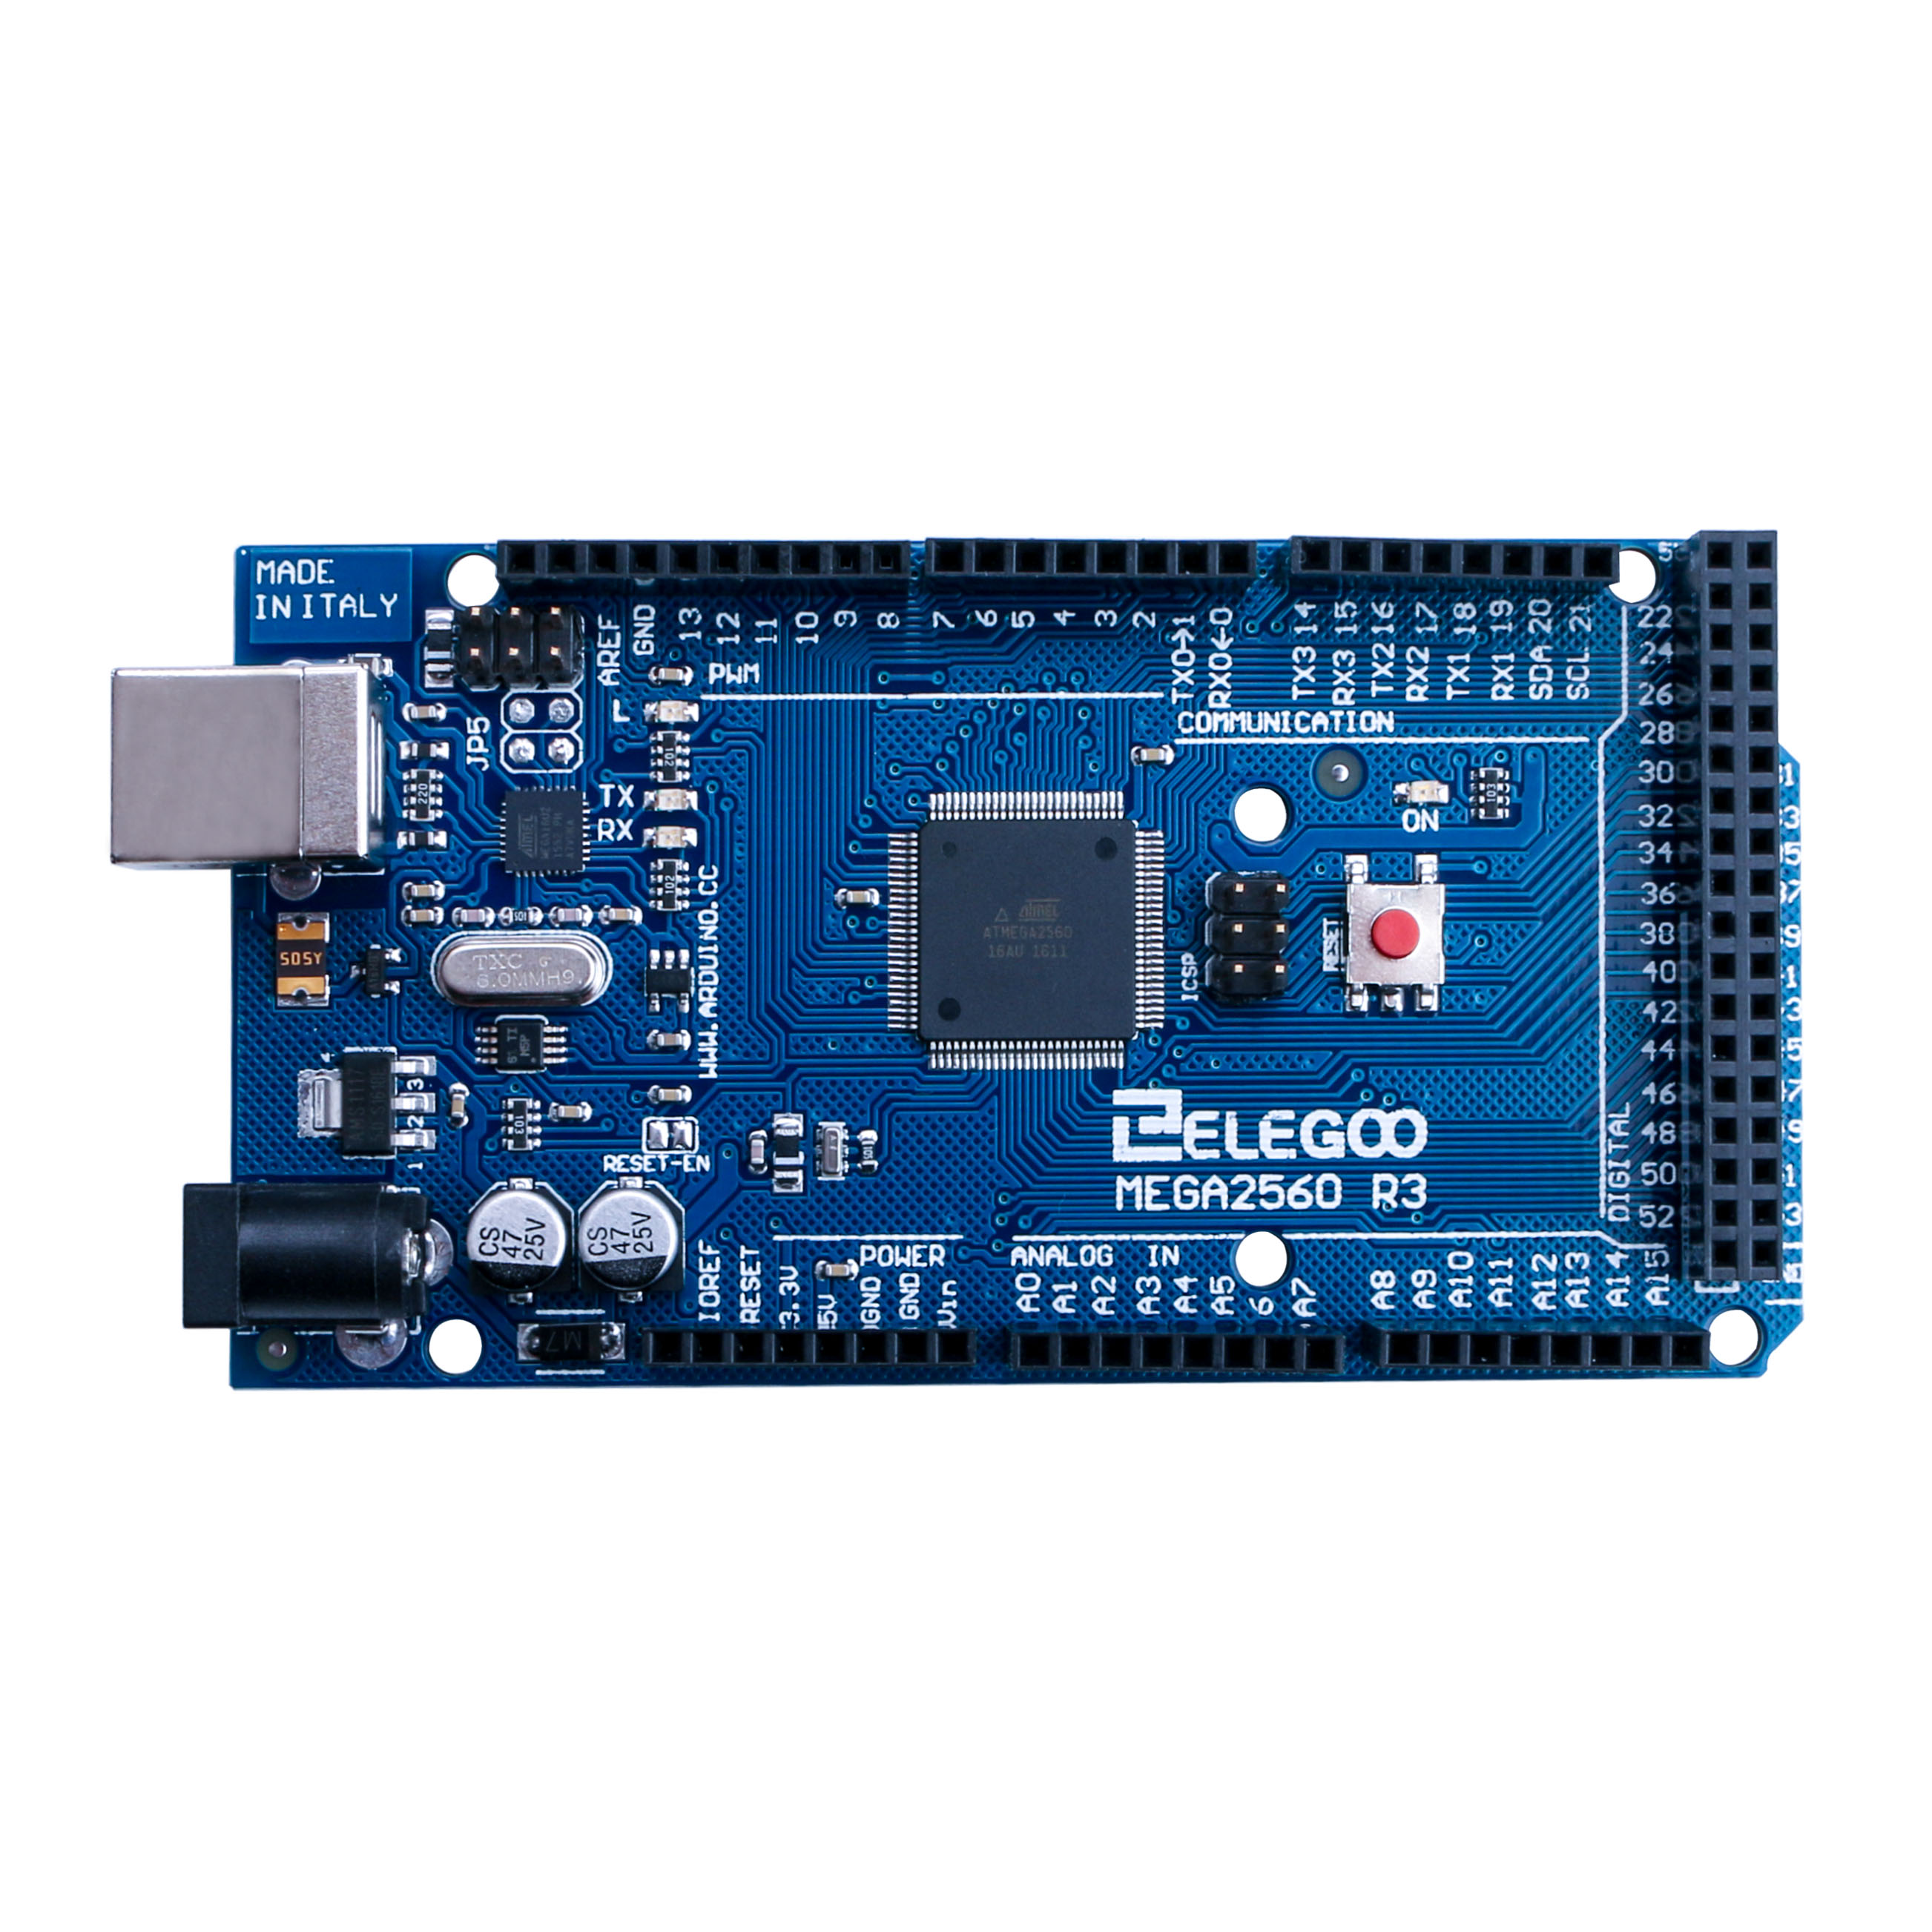
\includegraphics[width=0.4\textwidth]{imagenes/arduinomega.jpg}\\[1cm]
    \end{figure}
    
	\item \textbf{Pantalla LCD1602}
	\\
	Es el encargado de mostrar la visualización de la ejecución del programa principal, permitiendo de esta forma al usuario ser consciente en cada momento de las acciones que se están llevando a cabo en el sistema.
	\begin{figure}[h]
    \centering
    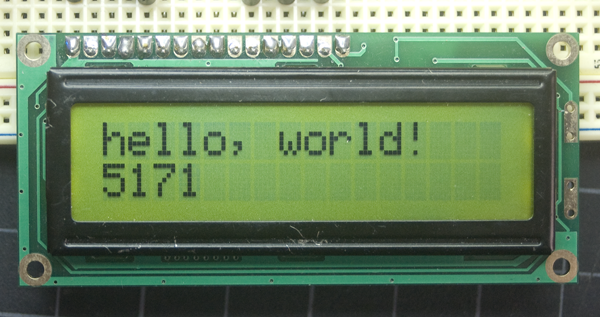
\includegraphics[width=0.4\textwidth]{imagenes/pantallalcd.png}\\[1cm]
    \end{figure}
    
	\item \textbf{Teclado matricial 4x4}
	\\
	Interfaz que actúa para ofrecer al usuario la capacidad de interactuar con la aplicación, para los juegos en dónde sea preciso su uso.
	\begin{figure}[h]
    \centering
    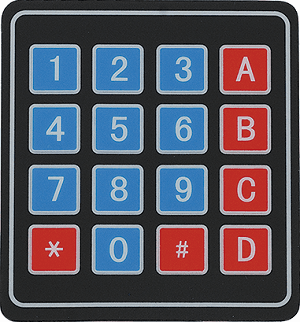
\includegraphics[width=0.3\textwidth]{imagenes/teclado4x4.png}\\[0.8cm]
    \end{figure}
    
	\item \textbf{Pulsadores de botón}
	\\
	Actúan también como interfaz entre el usuario y la aplicación, para los juegos dónde es necesario utilizarlos. 
	\item \textbf{Bombillas LED}
	\\
	Permiten la capacidad de ofrecer un estímulo visual al usuario para aumentar la capacidad de interacción entre este y la aplicación.
	
	\item \textbf{Resistencias y potenciómetro}
	\\
    Las resistencias son utilizadas para proteger diversos componentes del circuito y filtrar la corriente que circula por los elementos, evitando alteraciones o roturas por posibles subidas de tensión. El potenciómetro es necesario para controlar la tensión en la pantalla LCD y de esta forma conseguir el contraste óptimo para visualizar el contenido. 
\end{itemize}

\section{Software}



% Desarrollo del proyecto
%   1. Organización
%   2. Control de versiones
%   3. Hardware
%   4. Software
\chapter{Desarrollo del proyecto}
El presente capítulo expone todo lo relacionado con el desarrollo de este proyecto, las herramientas utilizadas para su organización y planificación, la gestión del software con su correspondiente control de versiones y la parte software.
\\

Para la parte hardware se muestran los componentes que constituyen el dispositivo prototipo, y razonando el uso de cada uno de ellos en las diferentes partes. También el diseño, simulación, y pruebas para el correcto funcionamiento del mismo.
\\

En la parte de software se explicará la estructura del programa desarrollado, explicando los algoritmos e implementación que permiten completar el diseño final.

\section{Organización}
En el desarrollo de un proyecto, la organización del mismo es un punto de vital importancia si se quiere completar con éxito. De esta forma, podemos fijar los objetivos que se pretenden cumplir y los niveles de prioridad de cada uno. También permiten localizar defectos que suceden durante el periodo de pruebas
\\

La gestión de las diferentes tareas a cumplir durante el desarrollo de un proyecto requiere de herramientas que nos permitan ver si los objetivos se cumplen. En este proyecto, se ha utilizado la plataforma Trello, que permite crear tableros de trabajo donde se añaden tareas, que se pueden mover entre listas que determinan si una tarea ya está realizada, se está realizando o aún está pendiente de realizar. De esta forma se facilita la organización del proyecto, tanto de forma individual como si se trabaja en equipo.
\\

La escritura de un informe final dónde se detallan los aspectos más relvantes del proyecto, es un punto vital para recoger la información e ideas desarrolladas. Esta memoria ha sido redactada mediante el sistema de composición de textos Latex con la plataforma Overleaf, que ofrece las herramientas para gestionar y ver el estado del documento de forma online, instantánea y gratuita. 
\\
\begin{figure}[h]
  \centering
  
\includegraphics[width=0.3\textwidth]{imagenes/overleaf.png}\\[1cm]
\end{figure}

\section{Control de versiones}
Para el desarrollo del software, es fundamental utilizar herramientas que permitan anotar cambios y llevar un control de desarrollo para poder realizar un diseño incremental. En este proyecto se ha utilizado Git, aprovechando el almacenamiento online que ofrece la plataforma GitHub. En el enlace \cite{GitProyecto} se encuentra la dirección asociada al repositorio de este proyecto.
\\

\begin{figure}[h]
  \centering
  
\includegraphics[width=0.3\textwidth]{imagenes/github.png}\\[1cm]
\end{figure}

\section{Hardware}
\subsection{Diseño y esquemático}
\subsubsection{Arduino general}
\subsubsection{Conexión con pantalla LCD}
\subsubsection{Conexión con teclado}
\subsection{Simulación}
\subsection{Montaje}

\section{Software}


% Resultados
\chapter{Resultados}
En este capítulo mostraremos los resultados obtenidos de este sistema basado en Arduino, la visualización del mismo y el funcionamiento sobre personas que sufren trastornos asociados a la dislexia.

% Planificación y recursos
\chapter{Planificación y recursos}
En el presente capítulo, se muestran la planificación realizada para el desarrollo de este proyecto, mostrando las diferentes etapas con las que transcurre y los costes materiales y humanos necesarios durante el diseño e implementación  para lograr cumplir el objetivo final.

\section{Etapas}

\section{Costes}

% Conclusiones
\chapter{Conclusiones}

\section{Valoración personal}

% Ampliaciones y mejoras
\chapter{Ampliaciones y mejoras}

\chapter{Elección de la plataforma de gestión documental}

Esta es una de las elecciones más significativas debido a que toda la gestión documental
y la manera en la que se realiza depende del software que utilicemos.
\\

En este caso en particular vamos a utilizar \textbf{Nuxeo} debido a que se adapta mejor a mis
necesidades que mi segunda opción, \textbf{Alfresco}.
\\

Los motivos por los que he elegido Nuxeo frente a Alfresco son los siguientes:

\begin{itemize}
	\item Alfresco sigue la filosofía \textit{Open Source} como método de trabajo, sino que la utilizan a modo de marketing
	 			ya que podemos comprobar que en su desarrollo solo intervienen trabajadores de dicha empresa a pesar de ser bastante
				más grande que Nuxeo.
	\item Alfresco tiene dos versiones, \textit{Community edition} y \textit{Commercial edition}. Esto no sería un problema
				si en la versión de la comunidad se incluyera \textbf{toda la funcionalidad}. Pero de esta manera, si quieres tener
				el software al compasdasdasdasdleto deberás pagar la versión comercial. Sin embargo, Nuxeo nos proporciona toda la funcionalidad
				base tengas o no tengas contasdasdasdasdcontasdasdasdasdratada una suscripción.
	\item La tecnología que impulsa Nuxeo es también de código libre y actual.
	\item La \textit{API} de Nuxeo es mucho más completa y sencilla, así como su documentación.
\end{itemize}


\begin{thebibliography}{0}
  \bibitem{Asandis} Asociación Andaluza de Dislexia: Guía general sobre dislexia 2010
  \bibitem{LaDislexia} http://www.ladislexia.net/causas-etiologia/
  \bibitem{WebConsultas} https://www.webconsultas.com/dislexia/tipos-de-dislexia-752
  \bibitem{GitDislexia} Victor Widell. Dsxyliea: https://geon.github.io/programming/2016/03/03/dsxyliea
  \bibitem{GitProyecto} https://github.com/jnavarro1412/TFG-II-2020
\end{thebibliography}

\thispagestyle{empty}

\end{document}
